%!TEX TS-program = xelatex
%!TEX encoding = UTF-8 Unicode
% Awesome CV LaTeX Template
%
% This template has been downloaded from:
% https://github.com/posquit0/Awesome-CV
%
% Author:
% Claud D. Park <posquit0.bj@gmail.com>
% http://www.posquit0.com
%
% Template license:
% CC BY-SA 4.0 (https://creativecommons.org/licenses/by-sa/4.0/)
%


%%%%%%%%%%%%%%%%%%%%%%%%%%%%%%%%%%%%%%
%     Configuration
%%%%%%%%%%%%%%%%%%%%%%%%%%%%%%%%%%%%%%
%%% Themes: Awesome-CV
\documentclass[]{awesome-cv}
\usepackage{textcomp}
\usepackage{graphicx}
%%% Override a directory location for fonts(default: 'fonts/')
\fontdir[fonts/]

%%% Configure a directory location for sections
\newcommand*{\sectiondir}{resume/}

%%% Override color
% Awesome Colors: awesome-emerald, awesome-skyblue, awesome-red, awesome-pink, awesome-orange
%                 awesome-nephritis, awesome-concrete, awesome-darknight
%% Color for highlight
% Define your custom color if you don't like awesome colors
\colorlet{awesome}{awesome-red}
%\definecolor{awesome}{HTML}{CA63A8}
%% Colors for text
%\definecolor{darktext}{HTML}{414141}
%\definecolor{text}{HTML}{414141}
%\definecolor{graytext}{HTML}{414141}
%\definecolor{lighttext}{HTML}{414141}

%%% Override a separator for social informations in header(default: ' | ')
%\headersocialsep[\quad\textbar\quad]
    \begin{document}
%%%%%%%%%%%%%%%%%%%%%%%%%%%%%%%%%%%%%%
%     Profile
%%%%%%%%%%%%%%%%%%%%%%%%%%%%%%%%%%%%%%
\begin{minipage}[b]{0.66666\textwidth}
\begin{center}
	\headerfirstnamestyle{Adrián} \headerlastnamestyle{Arroyo Calle} \\
	\vspace{2mm}
	{\faEnvelope\ adrian.arroyocalle@gmail.com} | {\faMobile\ +34 602 133 602} \newline {\faMapMarker\ Valladolid, Spain} {\faLink\ \url{http://adrianistan.eu}}
\end{center}
\end{minipage}
% FOTO
%\begin{minipage}[b]{0.33333\textwidth}
%	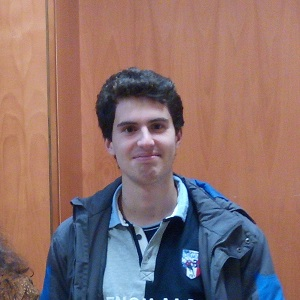
\includegraphics[width=0.8\textwidth]{stallman.jpg}
%\end{minipage}

%%%%%%%%%%%%%%%%%%%%%%%%%%%%%%%%%%%%%%
%     Education
%%%%%%%%%%%%%%%%%%%%%%%%%%%%%%%%%%%%%%
\cvsection{Education}
\begin{cventries}
	\cventry
	{BS in Computer Science}
	{Valladolid University}
	{Valladolid, Spain}
	{Unfinished}
	{}
\end{cventries}

\vspace{-2mm}
%%%%%%%%%%%%%%%%%%%%%%%%%%%%%%%%%%%%%%
%     Experience
%%%%%%%%%%%%%%%%%%%%%%%%%%%%%%%%%%%%%%
\cvsection{Experience}
\begin{cventries}
	\cventry
	{Internship}
	{Telefónica I+D}
	{Boecillo, Spain}
	{July 2019 - Present}
	{\begin{cvitems}
		\item {Internship at 4th Platform}
		\item {GitOps, Kubernetes, Docker}
	\end{cvitems}
	}
	\cventry
	{Treasurer}
	{BEST Valladolid}
	{Valladolid, Spain}
	{October 2018 - October 2019}
	{\begin{cvitems}
		\item {Manage finances of BEST Valladolid}
		\item {Be part of the ejecutive board}
		\end{cvitems}}
	\cventry
	{IT Coordinator}
	{BEST Valladolid}
	{Valladolid, Spain}
	{October 2017 – October 2018}
	{\begin{cvitems}
		\item {Coordinate the IT working group}
		\end{cvitems}}
	\cventry
	{Archaeologist voluntary}
	{Diputación Provincial de Soria}
	{Garray, Spain}
	{August 2017}
	{\begin{cvitems}
		\item {Work as a volunteer in the arqueological site of Numancia}
		\end{cvitems}}
\end{cventries}
\cvsection{Skills}
\begin{cventries}
	\cventry
	{}
	{\def\arraystretch{1.15}{\begin{tabular}{ l l }
		Programming languages:  & {\skill{ Rust, C, Python, Java, JavaScript, SQL, Prolog, Terraform}} \\
		Languages:  & {\skill{ Spanish (native), English ( FIRST B2)}} \\
		Software: & {\skill{Linux, Kubernetes, Docker, Azure, AWS, \LaTeX , PostgreSQL, Microsoft Office, Git}} \\
		\end{tabular}}}
	{}
	{}
	{}
\end{cventries}

\vspace{-7mm}
\cvsection{Projects}
\begin{cventries}
	\cventry
	{A blog mainly about programming in Spanish}
	{Blog Adrianistán}
	{Rust,JavaScript,Python}
	{http://blog.adrianistan.eu}
	{}
	\cventry
	{A puzzle game for web and mobile phones}
	{Anrokku}
	{TypeScript, Apache Cordova, Phaser}
	{}
	{https://play.google.com/store/apps/details?id=eu.adrianistan.anrokku}
	%\cventry
	%{Useful addons for Firefox and Thunderbird}
	%{firefox-addons}
	%{JavaScript}
	%{http://github.com/aarroyoc/firefox-addons}
	%{}
	%\cventry
	%{An opensource implementation of Free Cell solitaire for Haiku OS}
	%{SuperFreeCell}
	%{C++}
	%{http://github.com/aarroyoc/SuperFreeCell}
	%{}
	%\cventry
	%{A 3D voxel editor}
	%{Kovel}
	%{C++, wxWidgets, OpenGL}
	%{http://adrianistan.eu/kovel}
	%{}
	%\cventry
	%{A genetic algorithm to vectorize images}
	%{Mendel Vectorizer}
	%{Rust, Genetic Algorithm, Machine Learning}
	%{https://github.com/aarroyoc/mendel-vectorizer}
	%{}

	\vspace{-5mm}
\end{cventries}
\cvsection{Honors \& Awards}
\begin{cvhonors}
	\cvhonor
	{Winner of Special Mention at Open Data Contest Castille and Leon 2018}
	{Created Agromapa, an interactive visualization of agriculture in Castille and Leon}
	{Valladolid, Spain}
	{March 2019}
	\cvhonor
	{Winner of Catalysts Coding Contest Valladolid}
	{Competitive programming contest}
	{Valladolid, Spain}
	{March 2019}
	\cvhonor
	{Member of 62 SEMINCI (Valladolid Film Festival) Youth Jury}
	{Choosing the best film in Punto de Encuentro section}
	{Valladolid, Spain}
	{October 2017}
	\cvhonor
	{1st place at VallaHackaton 2017}
	{Created a game in two days about the theme \textquotedbl{}break\textquotedbl{}}
	{Valladolid, Spain}
	{May 2017}
	\cvhonor
	{Winner of \textquotedbl{}Las Matemáticas en el Planeta Tierra\textquotedbl{}}
	{Created a three dimensional raytracer to show how computer generated movies are}
	{Valladolid, Spain}
	{April 2016}
	\cvhonor
	{Finalist of Google Code-In contest}
	{Helped Haiku with apps and ports}
	{Mountain View, California}
	{February 2016}
	%\cvhonor
	%{Member of Spanish national orienteering team}
	%{Part of the school team that represented Spain in the World Championship}
	%{Antalya, Turkey}
	%{April 2015}
\end{cvhonors}
\ 
\end{document}